\graphicspath{{images/}}

\section{Vektorgeometrie}

\begin{definition}{Vektor}
    Objekt, das Betrag und Richtung hat.
    \begin{itemize}
        \item $\overrightarrow{0} = $ Nullvektor (Betrag = 0, einziger Vektor ohne Richtung)
        \item $\overrightarrow{e} = $ Einheitsvektor (Betrag = 1), evtl. mit Index $\vec{e_a}$
    \end{itemize}
    Vektoren werden durch Kleinbuchstaben mit einem Pfeil darüber bezeichnet ($\vec{a}$).
    Der Vektor, der den Punkt $P$ in $Q$ verschiebt, wird als $\vec{PQ}$ bezeichnet.
    Beschreiben zwei Vektoren dieselbe Translation (selber Betrag und Richtung),
    werden sie als gleich betrachtet.
    Es wird zwischen \textit{Orts-} und \textit{Richtungsvektoren} unterschieden.
\end{definition}

\begin{minipage}{0.6\linewidth}
    \begin{definition}{Gegenvektor}
        $-\vec{a}$ ist parallel zu $\vec{a}$, hat denselben Betrag,
        aber entgegengesetzte Richtung. 
    \end{definition}
    \end{minipage}
    \begin{minipage}{0.25\linewidth}
        {\small
        $$-\overrightarrow{a} = \begin{pmatrix}
            -a_x \\
            -a_y
            \end{pmatrix}$$}
    \end{minipage}
    \begin{minipage}{0.13\linewidth}
        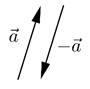
\includegraphics[width=1\linewidth]{vec-gegen.png}
    \end{minipage}

\begin{definition}{Länge/Betrag eines Vektors}
    $\abs{\vec{a}}=\sqrt{a_1^2+a_2^2+\cdots+a_n^2}$
\end{definition}

\begin{formula}{Berechnung Einheitsvektor/normieren}
    Gegeben: Vektor $\vec{a}$
    \begin{equation*}
        \vec{e_a}=\frac{1}{a}\cdot\vec{a} \quad = \quad \frac{\overrightarrow{a}}{|\overrightarrow{a}|}
    \end{equation*}
    Der Vektor $\vec{e_a}$ wird als \textbf{Einheitsvektor oder auch normiert} bezeichnet 
    und der Übergang von $\vec{a}$ nach $\vec{e_a}$ heisst \textbf{Normierung}.
\end{formula}



\begin{definition}{Orthogonal (Senkrecht)}
    Zwei Vektoren sind orthogonal, wenn der Winkel zwischen ihnen 90° beträgt. 
    $$\overrightarrow{a} \cdot \overrightarrow{b} = 0 \rightarrow \text{ orthogonal}$$
\end{definition}

\begin{definition}{Normalenvektor}
    Ein Normalenvektor, der orthogonal zu einer Ebene $E$ ist, heisst \textit{Normalenvektor} von $E$.
    Eine Koordinatendarstellung einer Ebene $E$ heisst normiert, wenn gilt: $\vec{n}=1$.
\end{definition}



\raggedcolumns

\paragraph*{Rechenregeln für Vektoren}

\begin{theorem}{Rechenregeln für Vektoren I}\\
    Für beliebige Vektoren $\vec{a}, \vec{b}$ und $\vec{c}$ gilt:
    \begin{center}
        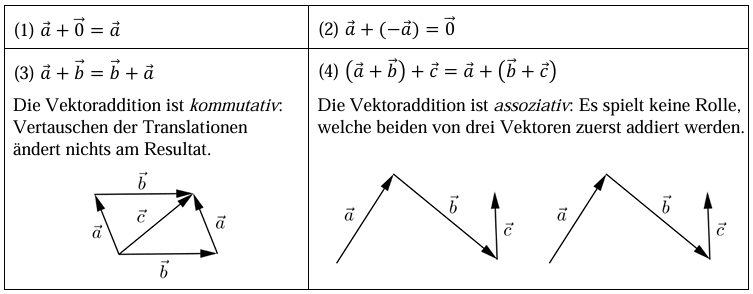
\includegraphics[width=1\linewidth]{vec-calc-regeln.png}
    \end{center}
\end{theorem}

\begin{theorem}{Rechenregeln für Vektoren II}
    \begin{itemize}
        \item $(-\lambda)\cdot\vec{a}=-(\lambda\cdot\vec{a})=\lambda\cdot(-\vec{a})$
        \item Assoziativ-Gesetz $\lambda\cdot(\mu\cdot\vec{a})=(\lambda\cdot\mu)\cdot\vec{a}$ 
        \item Distributiv-Gesetz $(\lambda+\mu)\cdot\vec{a}=\lambda\vec{a}+\mu\vec{a}$
        \item Distributiv-Gesetz $\lambda\cdot(\vec{a}+\vec{b})=\lambda\cdot\vec{a}+\lambda\cdot\vec{b}$
    \end{itemize}
\end{theorem}

\begin{minipage}{0.5\linewidth}
    \begin{formula}{Vektoraddition}\\
        $\overrightarrow{a} + \overrightarrow{b} = \begin{pmatrix} a_x + b_x\\ a_y + b_y \end{pmatrix}$
    \end{formula}
\end{minipage}
\begin{minipage}{0.5\linewidth}
\begin{formula}{Skalarmultiplikation}\\
    $\lambda \cdot \overrightarrow{a} = \begin{pmatrix}
    \lambda \cdot a_x \\
    \lambda \cdot a_y
    \end{pmatrix}$
\end{formula}
\end{minipage}

\raggedcolumns

\begin{formula}{Skalarprodukt} 
    $\overrightarrow{a} \cdot \overrightarrow{b} = a_x \cdot b_x + a_y \cdot b_y = |\overrightarrow{a}| \cdot |\overrightarrow{b}| \cdot \cos(\varphi)$
\end{formula}

\begin{theorem}{Wichtige Eigenschaften des Skalarproduktes}\\
    Für beliebige Vektoren $\vec{a}, \vec{b}$ und $\vec{c}$ und für jede beliebige Zahl $\lambda\in\R$ gilt:
    \begin{enumerate}
        \item $\vec{a}$ und $\vec{b}$ sind genau dann zueinander orthogonal (senkrecht), wenn $\vec{a}\cdot\vec{b}=0$.
        \item $\vec{a}\cdot\vec{a}=\abs{\vec{a}}^2$
        \item Kommutativ-Gesetz: $\vec{a}\cdot\vec{b}=\vec{b}\cdot\vec{a}$
        \item Distributiv-Gesetze: $\vec{a}\cdot(\vec{b}+\vec{c})=\vec{a}\cdot\vec{b}+\vec{a}\cdot\vec{c}$ und $(\vec{a}+\vec{a})\cdot\vec{c}=\vec{a}\cdot\vec{c}+\vec{b}\cdot\vec{c}$
        \item Gemischtes Assoziativ-Gesetz: $\lambda\cdot(\vec{a}\cdot\vec{b})=(\lambda\cdot\vec{a})\cdot\vec{b}=\vec{a}\cdot(\lambda\cdot\vec{b})$
    \end{enumerate} 
\end{theorem}

\begin{formula}{Winkelberechnung} {\small $\varphi$ = Winkel zwischen $\vec{a}$ und $\vec{b}$ ($0\le\phi\le\pi$)}
    $$\cos(\varphi) = \frac{\overrightarrow{a} \cdot \overrightarrow{b}}{|\overrightarrow{a}| \cdot |\overrightarrow{b}|} = \frac{a_x b_x + a_y b_y}{\sqrt{a_x^2 + a_y^2} \cdot \sqrt{b_x^2 + b_y^2}  } $$
\end{formula}

\begin{theorem}{Winkel und Skalarprodukt}

    \begin{wrapfigure}{r}{0.4\textwidth}
        \vspace{-20pt}
        \begin{align*}
            \phi<\frac{pi}{2},\, \text{ wenn } \vec{a}\cdot\vec{b} > 0 \text{ ist.}\\    
            \phi>\frac{pi}{2},\, \text{ wenn } \vec{a}\cdot\vec{b} < 0 \text{ ist.}\\    
            \phi=\frac{pi}{2},\, \text{ wenn } \vec{a}\cdot\vec{b} = 0 \text{ ist.}    
        \end{align*}
    \end{wrapfigure}
    Seien $\vec{a}$ und $\vec{b}$ zwei Vektoren und $\phi$ der eingeschlossene Winkel, 
    $0\leq\phi\leq\pi$, dann gilt:
    \vspace{40pt}
\end{theorem}



\begin{formula}{Vektorprodukt} $\overrightarrow{a} \times \overrightarrow{b}$ ist orthogonal zu $\overrightarrow{a}$ und $\overrightarrow{b}$

    \begin{minipage}{0.65\linewidth}
        $$\overrightarrow{a} \times \overrightarrow{b} = \left(\begin{array}{ccc}
            a_y \cdot b_z &-& a_z \cdot b_y \\
            a_z \cdot b_x &-& a_x \cdot b_z \\
            a_x \cdot b_y &-& a_y \cdot b_x
            \end{array}\right)$$
    \end{minipage}
    \begin{minipage}{0.3\linewidth}
        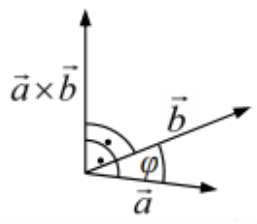
\includegraphics[width=0.7\linewidth]{vektorprodukt.png}
    \end{minipage}  
    
    \vspace{2mm}
    {\small
    $|\overrightarrow{a} \times \overrightarrow{b}| = |\overrightarrow{a}| \cdot |\overrightarrow{b}| \cdot \sin(\varphi) 
        \quad \overrightarrow{a} \times \overrightarrow{b} \neq \overrightarrow{b} \times \overrightarrow{a}$
    }
\end{formula}

\begin{theorem}{Eigenschaften des Vektorprodukt}\\
    Für beliebige Vektoren $\vec{a}, \vec{b}$ und $\vec{c}$ sowie für jede beliebiges $\lambda\in R$ gilt:
    \begin{itemize}
        \item $\vec{a}, \vec{b}$ \textbf{ sind genau dann kollinear, wenn } $\vec{a}\times\vec{b}=\vec{0}$
        \item $\vec{a}\times\vec{a}=\vec{0}$
        \item Antikommutativ-Gesetz: $\vec{a}\times\vec{b}=-(\vec{b}\times\vec{a})$
        \item Distributiv-Gesetz: $\vec{a}\times(\vec{b}+\vec{c})=\vec{a}\times\vec{b}+\vec{a}\times\vec{c}$
        \item Gemmischtes Assoziativ-Gesetz\\
            $\lambda\cdot(\vec{a}\times\vec{b})=(\lambda\cdot\vec{a})\times\vec{b}=\vec{a}\times(\lambda\cdot\vec{b})$ 
    \end{itemize}
    \begin{highlight}{<!>}
        Das normale Assoziativ-Gesetz gilt im Allgemeinen nicht ($\vec{a}\times(\vec{b}\times\vec{c})\ne(\vec{a}\times\vec{b})\times\vec{c}$)!
    \end{highlight}
\end{theorem}

\begin{formula}{Fläche des aufgespannten Parallelogramms}\\
    Der Betrag des Vektorproduktes $\vec{a}\times\vec{b}$ ist gleich dem Flächeninhalt des von 
        $\vec{a}$ und $\vec{b}$ aufgespannten Parallelogramms.\\
    \begin{minipage}{0.65\linewidth}
    $$h = |\overrightarrow{b}| \cdot \sin(\varphi)$$
    $$A = |\overrightarrow{a} \cdot h = |\overrightarrow{a} \times \overrightarrow{b}| = |\overrightarrow{a}| \cdot |\overrightarrow{b}| \cdot \sin(\varphi)$$
    \end{minipage}
    \begin{minipage}{0.3\linewidth}
        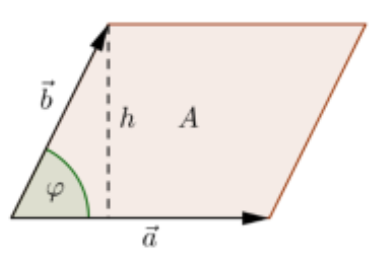
\includegraphics[width=0.9\linewidth]{parallelogramm.png}
    \end{minipage}
\end{formula}




    \begin{formula}{Orthogonal Projektion}von $\overrightarrow{b}$ auf $\overrightarrow{a}$\\
        \begin{minipage}{0.7\linewidth}
            \begin{align*}
                \vec{b}_a=\frac{\vec{a}\cdot\vec{b}}{\abs{\vec{a}}^2}\cdot\vec{a}   
                \text{ und }
                \abs{\vec{b}}_a=\frac{\abs{\vec{a}\cdot\vec{b}}}{\abs{\vec{a}}}   
            \end{align*}
        \end{minipage}
        \begin{minipage}{0.25\linewidth}
            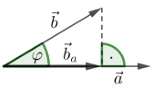
\includegraphics[width=0.9\linewidth]{vec-proj.png}
        \end{minipage}

        \vspace{1mm}
        
        Die erste Formel gilt für $0<\varphi\leq\frac{\pi}{2}$,
        die zweite für $\frac{\pi}{2}<\varphi\leq\pi$
    \end{formula}


\paragraph*{Lineare Abhängigkeit und Komponentendarstellung}

\begin{definition}{Lineare Abhängigkeit}
    Die Vektoren $\overrightarrow{a_{1}}, \overrightarrow{a_{2}}, \ldots, \overrightarrow{a_{k}}$ sind linear unabhängig, wenn gilt:
    \vspace*{2mm}
    \begin{itemize}
    \item $0 \cdot \overrightarrow{a_{1}}+0 \cdot \overrightarrow{a_{2}}+\cdots+0 \cdot \overrightarrow{a_{k}}$ ist die einzige Linearkombination, die $\overrightarrow{0}$ ergibt
    \item $\lambda_{1} \cdot \overrightarrow{a_{1}}+\lambda_{2} \cdot \overrightarrow{a_{2}}+\cdots+\lambda_{k} \cdot \overrightarrow{a_{k}} \neq \overrightarrow{0}(\lambda>0 \wedge \lambda \in \mathbb{R})$
    \end{itemize}
\end{definition}

\begin{definition}{Linearkombination}
    Gegeben sind $n$-Vektoren $\vec{a_1},\vec{a_2},\ldots,\vec{a_n}$.
    Der Ausdruck
    \begin{equation*}
        \lambda_1\cdot\vec{a_1}+\lambda_2\cdot\vec{a_2}+\ldots+\lambda_n\cdot\vec{a_n}
    \end{equation*}
    mit $\lambda_n\in R$ heisst \textit{Linearkombination} der Vektoren $\vec{a_1},\ldots,\vec{a_n}$.
\end{definition}


\begin{definition}{Komponentendarstellung}\\
    Jeder Vektor $\vec{a}$ kann als Linearkombination von $\vec{e}_1, \vec{e}_2,\ldots\vec{e}_n$
    eindeutig dargestellt werden. 
    Es gibt reelle Zahlen $a_1, a_2, \ldots a_n$ genannt (Komponente), so dass gilt:
    \begin{equation*}
        \vec{a}=a_1\cdot\vec{e}_1+a_2\cdot\vec{e}_2+\cdots+a_n\cdot\vec{e}_n=
        \begin{psmallmatrix}
            a_1\\a_2\\\vdots\\a_n
        \end{psmallmatrix}
    \end{equation*}
\end{definition}

\begin{definition}{Ortsvektor}\\
    Zu jedem Punkt $P$ des Vektorraums ist ein \textit{Ortsvektor} definiert
    \begin{equation*}
        \vec{r}(P)=\overrightarrow{OP}
    \end{equation*}.
    Ortsvektoren sind im Ursprung $O$ angeheftet und sind wie jeder Vektor Linearkombination 
    von $\vec{e_1}, \vec{e_2},\ldots, \vec{e_n}$ und lassen sich in Komponentenschreibweise darstellen:
    \begin{equation*}
        \vec{r}(P)=x_1\cdot\vec{e}_1+x_2\cdot\vec{e}_2,\ldots,x_n\cdot\vec{e}_n,\, \text{ also }
        \begin{psmallmatrix}
            x_1\\x_2\\\vdots\\x_n
        \end{psmallmatrix}
    \end{equation*}
\end{definition}

\begin{formula}{Komponentendarstellung von $\overrightarrow{OP}$}\\
    \vspace{-20pt}
    \begin{wrapfigure}{r}{0.3\textwidth}
        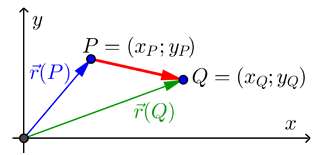
\includegraphics[width=\linewidth]{vec-komp-calc.png}
    \end{wrapfigure}
    \begin{align*}
        \vec{r}(Q)                      &=\vec{r}(P)+\overrightarrow{PQ}\\
        \Rightarrow \overrightarrow{PQ} &=\vec{r}(Q)-\vec{r}(P)=\begin{psmallmatrix}
            x_Q-x_P\\
            y_Q-y_P\\
            \cdots-\cdots
        \end{psmallmatrix}
    \end{align*}
\end{formula}

\begin{formula}{Rechnen mit Vektoren in Komponentendarstellung}\\
    Gegeben sind zwei Vektoren $\vec{a}=\begin{psmallmatrix}a_1\\a_2\\a_3\end{psmallmatrix}$
    und $\vec{b}=\begin{psmallmatrix}a_1\\a_2\\a_3\end{psmallmatrix}$ sowie ein $\lambda \in\R$.
    \begin{center}
        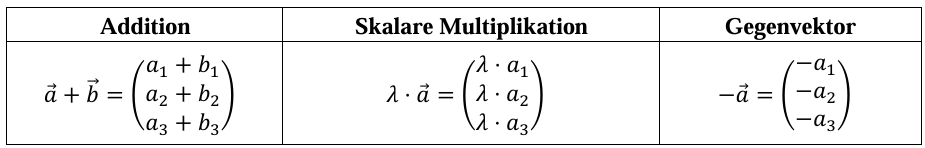
\includegraphics[width=\linewidth]{vec-komp-calc-regeln.png}
    \end{center}
\end{formula}



\raggedcolumns


\subsubsection*{Geraden und Ebenen}

\begin{definition}{Gerade}
    in der Ebene und im Raum\\
    \begin{minipage}{0.65\linewidth}
        \begin{itemize}
            \item $\overrightarrow{r}(A) = \overrightarrow{r}(P) + \lambda \cdot \overrightarrow{PQ}$
            \item $g: \overrightarrow{r}(P) + \lambda \cdot \overrightarrow{a}$
        \end{itemize}
    \end{minipage}
    \begin{minipage}{0.3\linewidth}
        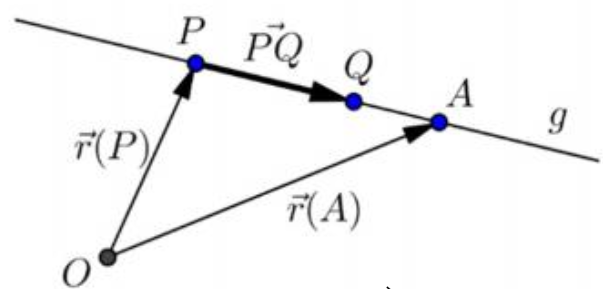
\includegraphics[width=0.9\linewidth]{gerade.png}
    \end{minipage}
    Der Punkt P heisst Aufpunkt, der Richtungsvektor $\overrightarrow{a}  = \overrightarrow{PQ}$ von g.
\end{definition}


\begin{definition}{Ebene}
    kann durch 3 Punkte festgelegt werden\\
    \begin{minipage}{0.65\linewidth}
    \begin{itemize}
        \item Die Vektoren $\overrightarrow{PA}$, $\overrightarrow{PR}$, $\overrightarrow{PQ}$ sind komplanar
        \item $\overrightarrow{PA} = \lambda \cdot \overrightarrow{PR} + \mu \cdot \overrightarrow{PQ}$
    \end{itemize}
    $$\overrightarrow{r}(A) = \overrightarrow{r}(P) + \lambda \cdot \overrightarrow{PR} + \mu \cdot \overrightarrow{PQ}$$
    \end{minipage}
    \begin{minipage}{0.3\linewidth}
        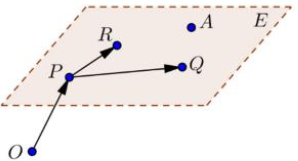
\includegraphics[width=1\linewidth]{ebene.png}
    \end{minipage}
\end{definition}

\paragraph*{Kollinear und Komplanar}   

\begin{theorem}{Lage} von Geraden im Raum\\
    \vspace*{2mm}
    %make a table to show the different cases
    \begin{tabular}{c|c|c|}
        & Gemeinsame Punkte & keine gem. Punkte \\
        \hline
        Kollinear & Identisch & echt Parallel \\
        \hline
        nicht kollinear & Schneidend & Windschief \\
        \hline
    \end{tabular}
\end{theorem}

\begin{definition}{Kollinear}
    
    \begin{minipage}
        {0.85\linewidth}
        Zwei Vektoren $\vec{a}$ und $\vec{b}$ heissen \textbf{kollinear}, 
        wenn es eine Gerade $g$ gibt, zu denen beide parallel sind. 
        Ein \textbf{Spezialfall} bildet dabei der Nullvektor, welcher zu jedem Vektor kollinear ist.
    \end{minipage}
    \hspace{1mm}
    \begin{minipage}{0.1\linewidth}
        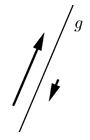
\includegraphics[width=\linewidth]{vec-kollinear.png}
    \end{minipage}
\end{definition}

\begin{theorem}{Eigenschaften kollinear Vektoren} $\vec{a}$ und $\vec{b}$\\
    so ist einer ein Vielfaches des anderen; 
    es gibt also eine reelle Zahl $\lambda$, sodass gilt: $\vec{a}=\lambda\cdot\vec{b}$
\end{theorem}



\begin{definition}{Komplanar}
    
    \begin{minipage}{0.8\linewidth}
        Drei Vektoren $\vec{a}$, $\vec{b}$ und $\vec{c}$ heissen \textbf{komplanar}, 
        wenn es eine Ebene $E$ gibt, zu denen alle drei parallel sind.
    \end{minipage}
    \hspace{1mm}
    \begin{minipage}{0.15\linewidth}
        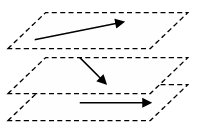
\includegraphics[width=\linewidth]{vec-komplanar.png}
    \end{minipage}
\end{definition}

\begin{theorem}{Eigenschaften komplanarer Vektoren}\\
    \begin{wrapfigure}{r}{0.2\textwidth}
        \vspace{-10pt}
        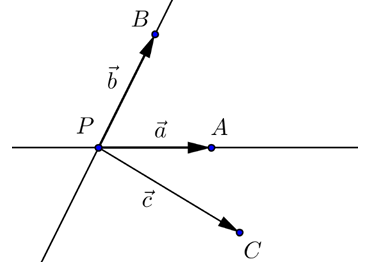
\includegraphics[width=\linewidth]{vec-kompl.png}
    \end{wrapfigure}
    Gegeben sind drei Vektoren $\vec{a}$, $\vec{b}$ und $\vec{c}$, für die gilt:
    \begin{itemize}
        \item $\vec{a}$, $\vec{b}$ und $\vec{c}$ sind komplanar.
        \item $\vec{a}$ und $\vec{b}$ sind nicht kollinear.
    \end{itemize} 
    Dann lässt sich $\vec{c}$ als Linearkombination von $\vec{a}$ und $\vec{b}$ darstellen; 
    es gibt also reelle Zahlen $\lambda$ und $\mu$, sodass gilt:
    \begin{equation*}
        \vec{c}=\lambda\cdot\vec{a}+\mu\cdot\vec{b}
    \end{equation*}
\end{theorem}

\begin{theorem}{Eigenschaften nicht komplanarer Vektoren}\\
    \begin{wrapfigure}{r}{0.2\textwidth}
        \vspace{-10pt}
        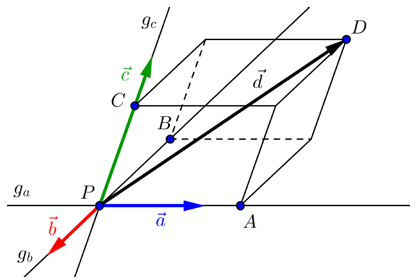
\includegraphics[width=\linewidth]{vec-nicht-kompl.png}
    \end{wrapfigure}
    Sind drei \textit{nicht komplanare} Vektoren $\vec{a}, \vec{b}$ und $\vec{c}$,
    dann lässt sich jeder Vektor $\vec{d}$ im $\R^3$ als Linearkombination von $\vec{a},\vec{b}$ und $\vec{c}$
    eindeutig darstellen;
    es gibt also reelle Zahlen $\lambda, \mu$ und $\nu$, so dass gilt:
    \begin{equation*}
        \vec{d}=\lambda\cdot\vec{a}+\mu\cdot\vec{b}+\nu\cdot\vec{c}
    \end{equation*}
\end{theorem}


\paragraph{Darstellungsformen von Ebenen und Geraden}

\begin{definition}{Parameterdarstellung}
    \begin{wrapfigure}{r}{0.3\textwidth}
        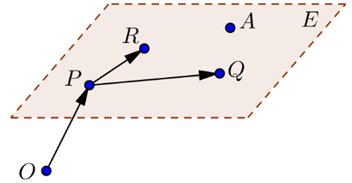
\includegraphics[width=0.9\linewidth]{vec-param.png}
    \end{wrapfigure}
    Eine Gerade oder Ebene $E$ lässt sich durch eine Gleichung der folgenden Form beschreiben:
    \begin{equation*}
        E:\,\vec{r}(P)+\lambda\cdot\vec{a}+\mu\cdot\vec{b}\, (\lambda,\mu\in\R)
    \end{equation*}
    Der Punkt $P$ heisst \textit{Aufpunkt}, die Vektoren $a=\overrightarrow{PQ}$ und 
    $\vec{b}=\overrightarrow{PR}$ heissen \textit{Richtungsvektoren} von $E$.
    Die Parameterdarstellung ist nicht eindeutig. Als Richtungsvektoren werden zwei beliebige
    Vektor gewählt, die \textit{parallel} zu $E$ sind und \textit{nicht kollinear} sind.
\end{definition}

\begin{definition}{Koordinatendarstellung}\\
    Eine Ebene $E$ im Raum lässt sich durch eine Gleichung der folgenden Form Beschreiben:
    \begin{equation*}
        E:\,ax+by+cz+d=0,\, \text{mit } a,b,c,d\in \R
    \end{equation*}
    Dait ist gemeint, dass die Ebene E aus allen Punkten $P$ besteht, deren Koordinaten
    $x, y$ und $z$ diese Gleichung erfüllen.
    Das $\abs{d}$ stellt den Abstand zum Ursprung dar, wenn die Gleichung normiert ist. 
    Ansonsten ist es $\frac{\vec{d}}{\vec{n}}$ 
\end{definition}

\begin{formula}{Umrechnung Parameterdarstellung zu Koordinatendarstellung}\\
    Für das Berechnen der Koordinatendarstellung aus der Parameterdarstellung gibt es mehrere
    Möglichkeiten.

    Die Einfachste ist das berechnen über den Normalenvektor aus dem Kreuzprodukt der Richtungsvektoren,
    welches die Koeffizienten $a, b$ und $c$ liefert.
    \begin{equation*}
        \vec{n}=\vec{a}\times\vec{b}=\begin{psmallmatrix}
            a\\b\\c
        \end{psmallmatrix}
    \end{equation*}
    Der Aufpunkt wird über das Einsetzen eines Punktes der Ebene $E$ ermittelt.

    Die zweite Möglichkeit ist es, ein LGS aufzustellen und die Parameter zu eliminieren.
    \begin{equation*}
        \vec{r}(P)+\lambda\cdot\vec{a}+\mu\cdot\vec{b}=\begin{psmallmatrix}
            x\\y\\z
        \end{psmallmatrix}
    \end{equation*}
\end{formula}

\begin{formula}{Umrechnung Koordinatendarstellung zu Parameterdarstellung}\\
    Um eine Koordinatendarstellung in eine Parameterdarstellung umzurechnen,
    werden drei Punkte berechnet.
    Einer dieser Punkte wird dann als aufpunkt gewählt und mit den restlichen
    werden Richtungsvektoren berechnet.
\end{formula}

\begin{concept}{Parameterdarstellung} der Ebene
    $$E: \overrightarrow{r}(P) + \lambda \cdot \overrightarrow{a} + \mu \cdot \overrightarrow{b}$$
    $$E: \overrightarrow{n} = \overrightarrow{a} \times \overrightarrow{b}$$
\end{concept}
    
\begin{example}
    $$E: 2x + 7y - 4z + 1 = 0$$\\
    Punkte einsetzen: $(0|0|z), (1|0|z), (0|1|z)$\\
    \begin{minipage}{0.5\linewidth}
    \begin{itemize}
        \item $2 \cdot 0 + 7 \cdot 0 - 4 \cdot z + 1 = 0 \Rightarrow z = \frac{1}{4}$
        \item $2 \cdot 1 + 7 \cdot 0 - 4 \cdot z + 1 = 0 \Rightarrow z = \frac{3}{4}$
        \item $2 \cdot 0 + 7 \cdot 1 - 4 \cdot z + 1 = 0 \Rightarrow z = \frac{8}{4}$
    \end{itemize}
    \end{minipage}
    \begin{minipage}{0.5\linewidth}
    $$E: \begin{pmatrix} 0 \\ 0 \\ \frac{1}{4} \end{pmatrix} +
    \lambda \begin{pmatrix} 1 \\ 0 \\ \frac{2}{4} \end{pmatrix} +
    \mu \begin{pmatrix} 0 \\ 1 \\ \frac{7}{4} \end{pmatrix}$$
    \end{minipage}
\end{example}

\begin{concept}{Koordinatendarstellung} der Ebene
    $$E: ax + by + cz + d = 0$$
    $$\vec{n} = \begin{pmatrix} a \\ b \\ c \end{pmatrix}, \quad
    \vec{n} \perp \begin{pmatrix} x \\ y \\ z \end{pmatrix}, \quad
    \begin{pmatrix} x \\ y \\ z \end{pmatrix} \cdot \begin{pmatrix} a \\ b \\ c \end{pmatrix} = 0$$
\end{concept}

\begin{example}
    $$E: \begin{pmatrix} 2 \\ 4 \\ 1 \end{pmatrix} + \lambda \cdot \begin{pmatrix} 1 \\ 3 \\ 1 \end{pmatrix} + \mu \cdot \begin{pmatrix} 2 \\ 2 \\ -4 \end{pmatrix}$$
    $$\vec{n} = \begin{pmatrix} 1 \\ 3 \\ 1 \end{pmatrix} \times \begin{pmatrix} 2 \\ 2 \\ -4 \end{pmatrix} = \begin{pmatrix} -12 -2 \\ 2 + 4 \\ 2 - 6 \end{pmatrix} = \begin{pmatrix} -14 \\ -6 \\ -4 \end{pmatrix}$$
    $$E: -14x - 6y - 4z + d = 0$$
    Aufpunkt einsetzen: $-14 \cdot 2 - 6 \cdot 4 - 4 \cdot 1 + d = 0 \Rightarrow d = 8$
\end{example}

\paragraph*{Abstände berechnen}


\begin{formula}{Abstand Punkt-Gerade}\\
    Für das finden des Abstandes zu einer Geraden gibt es verschiedene Möglichkeit.\\
    \textbf{Hier der Weg über den Fusspunkt.}
    Gegeben Gerade $g=\vec{r}(P)+\lambda\cdot\vec{a}$ in Parameterform und Punkt $A$. Gesucht ist der Fusspunkt $B\in g$.
    \begin{wrapfigure}{r}{0.3\textwidth}
        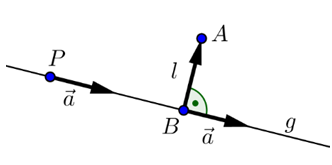
\includegraphics[width=0.8\linewidth]{vec-abstand-von-punkt.png}
    \end{wrapfigure}
    \begin{enumerate}
        \item Da $B\in g\Rightarrow \vec{r}(B)=\begin{psmallmatrix}
            P_x+a\lambda_B\\
            P_y+b\lambda_B\\
            P_z+c\lambda_B
        \end{psmallmatrix}$. 
        \item Da $\overrightarrow{BA}\perp g\Rightarrow\overrightarrow{BA}\cdot\vec{a}=0$
        \item Jetzt kann ein LGS aufgestellt und aufgelöst werden.
    \end{enumerate}
    Weiter Möglichkeit gehen über die Projektion oder die Fläche des Kreuzprodukt.
\end{formula}

\begin{formula}{Abstand Punkt-Ebene}
    \begin{wrapfigure}{r}{0.3\textwidth}
        \vspace{-10pt}
        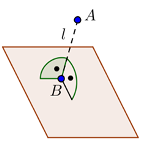
\includegraphics[width=0.7\linewidth]{vec-abstand-von-ebene.png}
        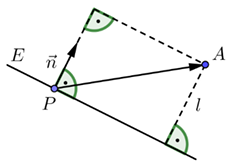
\includegraphics[width=0.7\linewidth]{vec-abstand-von-ebene2.png}
    \end{wrapfigure}
    Gegeben ein Punkt $A=(x_A;y_A;z_A)$ sowie eine Ebene $E$ mit der \textbf{normierten} 
    Koordinatendarstellung $E:\,ax+by+cz+d=0$.
    Dann gilt für den Abstand $l$ des Punktes $A$ von der Ebene $E$ die gleichung (1).
    Ist die Koordinatendarstellung nicht \textbf{nicht normiert}, so gilt (2).
    \begin{align}
        l=\abs{ax_A+by_A+cz_A+d}\\
        l=\frac{\abs{ax_A+by_A+cz_A+d}}{\abs{\vec{n}}}
    \end{align}
\end{formula}

\begin{KR}{Abstand Punkt-Gerade}
    \begin{enumerate}
        \item $\overrightarrow{BA} = \overrightarrow{r}(A) - \overrightarrow{r}(B)$
        \item $0 = \overrightarrow{BA} \cdot \overrightarrow{a}$
        \item Length $= |\overrightarrow{BA}| = \frac{|\overrightarrow{PA} \times \overrightarrow{a}|}{|\overrightarrow{a}|}$
    \end{enumerate}
\end{KR}

\begin{example}
    $$g: \begin{pmatrix} 1 \\ 13 \end{pmatrix} + \lambda \begin{pmatrix} 3 \\ 5 \end{pmatrix}, \quad A(3|-1)$$
    \begin{minipage}{0.65\linewidth}
    \begin{enumerate}
        \item $\overrightarrow{BA} = \vec{r} \cdot \begin{pmatrix} 3 \\ -1 \end{pmatrix} - \vec{r} \cdot \begin{pmatrix} 1 + 3 \lambda \\ 13 + 5 \lambda \end{pmatrix}$
        \item $0 = \begin{pmatrix} 3 - 1 - 3 \lambda \\ -1 - 13 - 5 \lambda \end{pmatrix} \cdot \begin{pmatrix} 3 \\ 5 \end{pmatrix} \rightarrow \lambda = x$
        \item Length $ = \left| \begin{pmatrix} 2 - 3x \\ -14 - 5x \end{pmatrix} \right|$ 
    \end{enumerate}
    \end{minipage}
    \begin{minipage}{0.3\linewidth}
    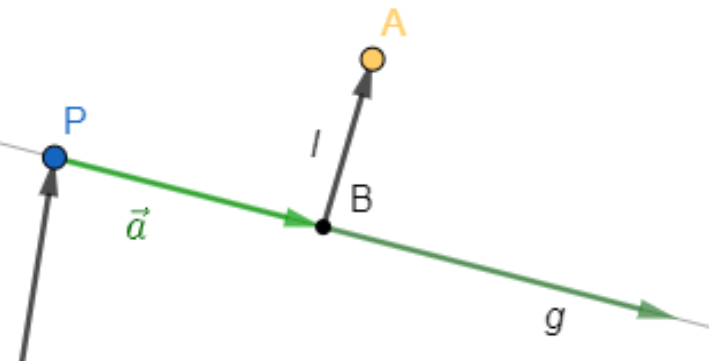
\includegraphics[width=1\linewidth]{abstand.png}
    \end{minipage}
\end{example}

\begin{KR}{Abstand Gerade-Gerade}
    \begin{enumerate}
        \item $\overrightarrow{BA} = \overrightarrow{r}(A) - \overrightarrow{r}(B)$
        \item $\overrightarrow{a} \times \overrightarrow{b} = \overrightarrow{n}$
        \item Length $= \frac{|\overrightarrow{BA} \cdot \overrightarrow{n}|}{|\overrightarrow{n}|}$
    \end{enumerate}
\end{KR}

\begin{KR}{Abstand Punkt-Ebene}
    \begin{enumerate}
        \item $\overrightarrow{BA} = \overrightarrow{r}(A) - \overrightarrow{r}(B)$
        \item $0 = \overrightarrow{BA} \cdot \overrightarrow{n}$
        \item Length $= |\overrightarrow{BA}| = \frac{|\overrightarrow{PA} \cdot \overrightarrow{n}|}{|\overrightarrow{n}|}$
    \end{enumerate}
\end{KR}











